\chapter{Introduction}
\label{chap:introduction}

% intro
Software has become pervasive and integrated with numerous platforms and applications such as mobile devices, web sites, embedded systems, safety critical systems. Creating and managing a software application can be time consuming and resource intensive. The development of software applications commonly integrate the usage of \gls{vcs} to manage the application by storing the current version as well as previous versions in a repository. The development of a repository is limited by the resources available to the team developing the application. Effective allocation of these limited resources could be the deciding factor in whether repository will be successful or not. Furthermore, a \gls{vcs} manager such as GitHub could leverage repository resource allocation for managing the resources provided to repositories hosted by them.

% TODO summarize relevant research about change prediction/resource allocation.

Previous works in change prediction include Bantelay, Zanjani and Kagdiw who studied evolutionary coupling to create predictions of commit and interactions within a repository\cite{Bantelay2013}. Giger, Pinzger and Gall analyze an approach for predicting the type of change that will occur\cite{Giger2012}. Hassan and Holt predict change propitiation of a purposed change\cite{Hassan2004}. Kagdi and Maletic outline an approach for predicting software changes through a dependency analysis of the repository history\cite{Kagdi2007}. Ying, Murphy, Ng and Chu-Carroll create a method for predicting source code changes given a change within the repository\cite{ying2004}. The predictions are made by identifying elements within the repository that are associated through frequent co-changes. We hope to build on previous research to provide change predictions to help improve resource allocation for both repository developers as well as \gls{vcs} managers.


% providing people with an easy to use device that is always close by. Developers are also able to create applications which can reach a wider audience through the use of application market places such as the Google Play Store, Apple App Store. In other cases such as web development system are expected to be working constantly. The applications must provide maximum availability with minimal number of issues as possible. Developing large scale applications is a difficult task that when executed incorrectly can lead to massive losses for all parties involved in the project. 
% % TODO maybe mention the number of projects that typically fail.

% The software development process can be time consuming and costly even if the project is successful. During the development of a project, a large number of changes will be applied to the original source code. These changes can introduce features, issues or fixes to the project. Further still, projects will often have multiple developers contributing. Managing the changes made to a project is often managed by a \gls{vcs}. A \gls{vcs} will store the change data and help facilitate the collaboration between different developers. Predicting where changes will occur within the project could help developers of a project keep track of sections of the software project that need more attention. The data may also promote a reflection on the design of the section to improve the software project.

\section{Objective \& Methodology}

% Possible reduce.
%This research is vital to improving the development process of software projects.
The mining of open source software repositories is widely used to help research into various software topics relating to software development and quality assurance. Research can provide improvements to the development process of software repositories. With an improved development process, more repositories may succeed in accomplishing their outlined goal. The process of developing a repository will of course take time to complete. The time for a repository to be completed relies on numerous factors including scope, man power, experience. Over the course of development, changes will be made to repository. Changes can be made to almost any part of the repository including design, number of developers and type of developers. These changes will in most cases have a measurable impact on the repository. In case of adding more developers, the intended result may be to increase functional capabilities within a shorter span of time. Even with an intended result, the actual result may differ and should be measured to determine the effectiveness of a given change.

Development of a software application will attempt to solve any number of problems. A few examples of typical software problems are; video games, telecommunication or financial. The success of an application however does not rely on a single factor. Software applications may fail in many different ways affecting the scope, cost, or timeliness of the project. Furthermore, software development often continues long after the product is delivered to clients. Managers or developers may decide to increase the resources available for the development in an attempt to solve the problem. Without clear understanding or knowledge of what resources are necessary can exacerbate the problem. For example, allocating more developers to work on a project will also require more coordination between developers which can increase overhead. Providing  predictions of upcoming code changes can provide developers and managers insight into the development schedule of their application and help them make more informed decisions regarding future resource allocation.

The developers of the repository should manage the growth of the repository to ensure that the changes that are made result in an expected outcome. Keeping track of every change to a repository can be difficult because of external changes which are beyond the control of the developers. However, for the majority of the changes within the repository they are kept track through \gls{vcs}. With proper use of a \gls{vcs}, the important changes made to the repository available. This can help keep previous releases of the software available or even help resolve a bug that was introduced in a recent change. Furthermore, developers have control over what is stored in the \gls{vcs} allowing for granularity based on developer preferences. With numerous developers, a \gls{vcs} can also help improve how these developers interact and share the changes they made. Some commonly used \gls{vcs} include Git \footnote{\url{https://git-scm.com/}}, \gls{svn}\footnote{\url{https://subversion.apache.org/}} and Mercurial\footnote{\url{https://www.mercurial-scm.org/}}.

The impact of changes can be measured and provides insights into how the repository changes. However first the data must be collected, processed and stored. While changes may occur in various forms, a more accessible one would be the source code changes in the software repository. These changes are very fine grain since they will account for almost all functionality changes with the repository. The only functionality changes not accounted by source code would be external changes (e.g. library changes). Changes will map to functionality changes that provide fixes, new functionality, or removal of functionality. The source code changes will provide a large amount of noise since every change is included. This excessive granularity can make tracking the desired changes more difficult. Visualization of the data collected allows for a more accessible look at the data to provide potential insights.


% TODO talk about project development
% - limited time
% - project costs
% - open source difference

As discussed earlier, there are two main types of software repositories that are developed, either closed source or open source. \gls{oss} repositories will generally provide access to the source code, the ability to change and finally redistribute the changes. \gls{oss} is widely used in developing software repositories of various sizes and scope. In these repositories developers are able to contribute towards the a repository that is often used by a wider audience. While smaller \gls{oss} repositories may have a small number of developers, larger repositories can contain developers from numerous locations around the world contributing at different times. The development of \gls{oss} is often the focus of research related to software development since the repositories are open and freely available. The authors are able to publish and use the data as they wish since it is publicly available. There are also countless \gls{oss} repositories to study and investigate.

The collection of data is done through data mining. Data mining is the act of collecting data from one or more sources to use for another goal. Often data mining will use a data source not traditionally used, since the goal of data mining is to extract and use information. The actual use of the data once collected can vary greatly from visualizing to modeling. Data can also be collected in several forms including continuous streams of data, sporadic data and one time collection. Depending on what type of data is being collected and the purpose of the collection the means of collection may also vary. Another concern related to data mining is that of Big Data. If a source provides a wealth of data, then extra measures should be taken to manage the size of the data set. Without diligent management, a data set can become unwieldy with massive overhead that are entirely avoidable.

% machine learning
The goal of the approach is to predict changes that will occur within the repository using the commit history. In this case machine learning techniques are leveraged to create a model based on the data collected through mining GitHub to predict changes. Machine learning techniques are widely used to support the completion of difficult tasks that involve patterns. A machine learning algorithm is generally an algorithm that attempts to detect and mimic patterns within a data set. There are many different types machine learning algorithms including:

% Table of ML algorithms
\begin{enumerate}
\item Support Vector Machine (SVM)
\item Random Forest (RF)
\item Artificial Neural Network (ANN)
\item Deeplearning Artificial Neural Network (ANN)
\item Regressors
\item Bayes Na{\"i}ve Classifiers (BNC)
\end{enumerate}

Each technique provides advantages and disadvantages depending on the purpose and the data set in use. The primary focus will be on \gls{svm} and \gls{rf} since they are used as part of the proposed work. These two machine learning algorithms were selected because of their wide use in existing works. Specifically, research related to data mining often employed these techniques to make use of the collected data. Regardless of the predictive model, the training and testing layout is the same, by sampling a subset from the data source to use towards training of the model. To test the model a second subset that is distinct from the first is retrieved to permit the performance of the model to be measure.

\gls{svm} is an algorithm that attempts to classify data into two distinct categories. This algorithm is a supervised learning technique that requires a training data set to build the categorization model. The training set will consist of data samples from each classification as well as which classification the data sample belongs to. After creating the model for a \gls{svm} new data vectors can be provided to the model and be classified into one of the two categories. The model will be constructed by attempting to linearly separate the data into two distinct groups. If the data cannot be separated linearly, then the data is mapped to a higher dimension to allow for proper separation. During the separation of data points into two groups, the model may reclassify data points in an attempt to fix errors within the data set. This feature allows for some error to be present within the training set without causing further errors. In the case that points which are valid are detected as errors then the separation has generated errors and the features or data used may not be useful towards making a prediction.% TODO maybe talk about wide use of svms in research and industry?

\gls{rf} is another supervised learning technique that requires a training data set to create an prediction model. The origin of random forests is the decision tree learning method. A single decision tree creates a tree structure where each internal node in the tree represents a decision where in the final destination is the outcome. \gls{rf} extends decision trees to address the tendency for a decision tree to overfit the data. A \gls{rf} uses numerous decision trees as well as a modified version of bootstrap aggregation to get more robust predictions.

% TODO create an image of a simple decision tree

	% TODO explain svm and rf in further details.

The machine learning algorithm makes use of the training data to create a model for predicting the classification of a given value. An analysis of change data can help in the selection of useful information for creating the predictive model. The data is collected from the repository's historical data that can provide a large data set to work with. Managing the data and selecting ideal samples for training must be considered to provide a strong predictive model.

\begin{figure}[t]
    \centering
        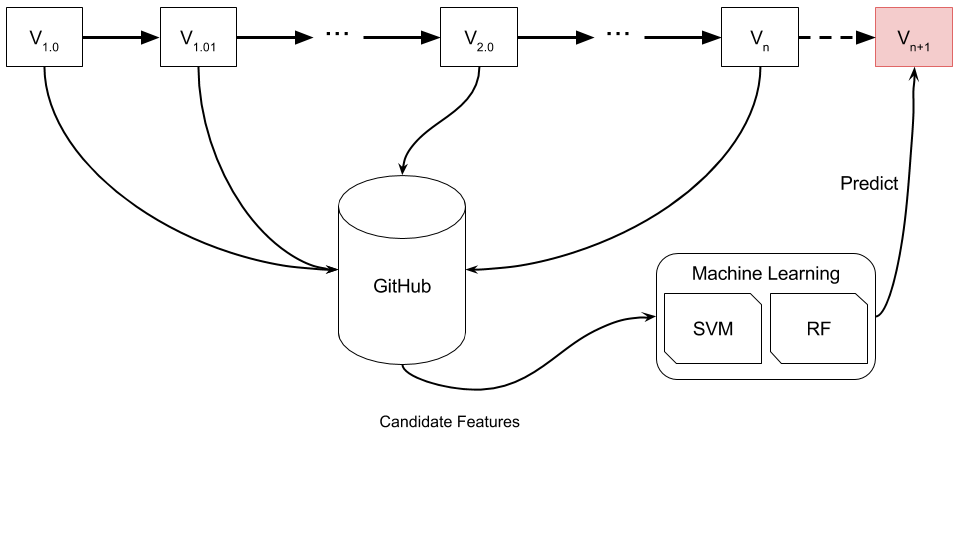
\includegraphics[width=1.0\textwidth]{images/overview}
    \caption{Approach Overview}
    \label{fig:overview}
\end{figure}

% TODO either remove or re-write this.
%This thesis generally covers topics relating to effort estimation and planning of project development. The development of a software project can vary greatly based on the scope of the project. Larger scale project that have a complex task or set of tasks to accomplish often require a long period of time with a committed team of developers. Even once a project completely performs a task further development is needed to maintain the project for the remainder of its life.
%For the development of software in a commercial setting the ability for managers to identify the cost of a project is essential for effective business decisions. Effort estimation is one possible avenue for project managers to leverage to identify the complexity of a project and associated cost of that project. 
%The ability of developers or managers to extract more information from a project is essential to helping them make more informed decisions about the development of the project. For example if a developer can identify a location within a project that is very likely to receive changes in future development then the development may be more inclined carefully consider the types of changes necessary to make.

% TODO talk about the role of visualization?

% Thesis statement
We propose a tool that assists in managing the development of software repositories by predicting changes that are likely to occur. This work explores leveraging change prediction of the source code using the commit history to assist in the development of \gls{oss} scale repositories. The key factors; sampling size, feature set and data balancing are investigated using the tool to provide a deeper understanding the feasibility of the tool. Several \gls{oss} repositories were selected to conduct experiments to determine the impact of each of the factors.

\section{Contributions}

% Contributions
Our contributions are in mining of \gls{oss}, visualization of a repository's change history, machine learning change prediction, data collect which can be used and extended. Providing clear and accessible visualizations allows for the development data to be inspected more thoroughly. Likewise, strong predictions of change can assist in the development of more robust, efficient and less costly software programs. Finally, the collection of historical data for use of predicting future changes is presented as a possible option when predicting future changes within a repository.

There are several different areas where this work can be applied and provide improvements. The main area which this research is applicable would be that of software development by providing support during the development process. The prediction of future changes within a repository are made available to developers to support them when choosing tasks or making new changes to the repository. With the knowledge of where changes are likely to occur within the repository developers may be more prepared in making such changes. This is especially true if this work was extended to provide more specific change information about future changes. Another potential use for this approach would be in resource allocation for software repository development. A larger repository with numerous developers contributing will require each developer to work on various task an attempt to limit conflicting contributions. With the ability to predict where future changes will likely occur developers can coordinate more effectively with other developers mange interactions and overlap. Finally, the approach could help with resource allocation for a \gls{vcs} provider, such as GitHub. A \gls{vcs} could use the repository data to efficiently allocate resources based change predictions for each repository. If a repository is likely of have near future changes then more resources are necessary for that repository compared to one that is less likely to receive changes in the near future. With strong predictions a system could be more effectively managed and offer savings to the company.

\section{Organization}
% Organization

The remainder of the thesis is organized into 5 more chapters.

\begin{enumerate}
\item \hyperref[chap:related_works]{Literature Review} which provides more details related to the foundation of this work. Primarily this chapter will cover the data that is collected for the analysis.
\item \hyperref[chap:visualization]{Visualization of Commit Data} discusses how the data is collected, stored and visualized.
\item \hyperref[chap:prediction]{Prediction of Commit Data} outlines the data and methods that are used to predict change within a repository.
\item \hyperref[chap:experiments]{Experiments} reports the experiments conducted and their results.
\item \hyperref[chap:conclusions]{Conclusion} summarizes the results and contributions and proposes future work to build of the thesis.
\end{enumerate}

